% Chapter Template

\chapter{Secure Neighbour Discovery Protocols} % Main chapter title

\label{Chapter4} % Change X to a consecutive number; for referencing this chapter elsewhere, use \ref{ChapterX}

\lhead{Chapter 4. \emph{Secure Neighbour Discovery Protocols}} % Change X to a consecutive number; this is for the header on each page - perhaps a shortened title

%----------------------------------------------------------------------------------------
%	SECTION 3
%----------------------------------------------------------------------------------------

We have already presented a set of device pairing protocols and formally analysed them at the previous chapters. Basically, by adapting human assistance, wireless devices can establish secure connections among them. Before this stage, each device must know existence of its partners. The ability to determine the existence of participants within physical range in many systems from cellular infrastructure-based networks, wireless local area network to sensor networks, and short range wireless technologies is fundamental ranging problem. Thus, security mechanisms for ranging protocols should be seriously considered. Particularly, a secure ranging protocol must validate correctly both distance between participants and identification of participants. 

One potential threat is that due to varieties of wireless interfaces with different signal power, false results from distance ranging and validating processes in many neighbour discovery mechanisms might appear. The threat is an old-school problem in traditional wireless networks, but it becomes serious in distributed wireless systems with heterogeneous devices. Attackers can take advantage to generate false connections, that significantly reduces stability and security of the systems. This has not mentioned before. 

We put ourselves deeply between these problems, and find that time-based, or location-based neighbour discovery protocols cannot obtain correctly ranging goals. Additionally, some of them were exploited at the connection validating process. Meanwhile, current formal verification reasoning about security neighbour discovery protocols cannot resolve the problems. This motivates us to study more secure neighbour discovery mechanisms in context of Internet of Things where a huge amount of heterogeneous devices are inter-operating. 

Contributions of this chapter are following:
\begin{enumerate}
\item We present existing neighbour discovery protocols, address their limitations, and present some incorrect existing protocols.  
\item We adapt our formalisation on Strand Spaces with some extensions on physical characteristics and some helpful propositions to deal with communication statuese among principals. 
\item Our model allows us obtain a notable result. We prove that time-based or distance-based neighbour discovery schemes cannot confidentially achieve their goals due to difference of physical signal power of principals. 
\end{enumerate}

Chapter 4 begins with a comprehensive survey of current proposals of secure neighbour discovery techniques, and vulnerabilities. We then present some incorrect protocols and conduct correct one. We introduce formalisation based on Strand Spaces in the next part. An analysis of ADVSIG~\cite{Raffo:2004:ASS:1029102.1029106} protocol concludes this chapter. 
 
 \section{Overview on Neighbour Discovery Protocols}

Neighbour discovery is the process by which a device in a network determines the number and identity of other in its vicinity. In wireless context, neighbours of a device are usually defined as ones that lie within its radio range. Devices considered as neighbours may cooperate in the performance of various tasks such as communications, sensing, and localisation. For instance, in perfect environment with no obstacle and noise, a device can determine its honest neighbours using flying time measurement. Particularly, a device, called $A$, broadcasts a greeting message to a potential device, called $B$, then $B$ replies to $A$ quickly after receiving this message. Afterwards, when completely observing the feed-back message, $A$ measures the time-of-flight, and multiplies it by signal propagation speed in current medium to obtain the distance. If distance is lower than a pre-defined threshold, $A$ concludes that $B$ is its neighbour. 

In this chapter, we need to explicitly distinguish between different types of links. A link is a generic term denoted a relationship between two participants. There are two kinds of links: \emph{logical} and \emph{physical}. While a logical link describes existence of path of a message from one strand to another, a physical one describes a directional and physical path without any relaying point from one strand to another one. Moreover, each type of link has two states: \emph{unidirectional} and \emph{bidirectional}. In one hand, a \emph{unidirectional} link from $A$ to $B$ states that $B$ can receive messages from $A$, but $A$ cannot receive messages from $B$. In the other hand, a \emph{bidirectional} link from $A$ to $B$ states 
that $A$ and $B$ can receive messages from each other. 

Neighbour discovery protocols are apparently vital parts in current systems. Nevertheless, these protocols in wireless environment are easily abused by malicious activities of attackers. Tackling this problems, many approaches for securely discovering neighbours have been proposed. 

In this session, we present some applications of neighbour discovery, their threats and vulnerabilities. Then we recap existing secure approaches in categories.

\subsection{Neighbour Discovery Applications}

Neighbour discovery protocol is discovered under a form of a principal part of many applications such as physical authentication, network authentication, routing built-up, and localisation. This following examples are referred from~\cite{Marcinthesis}.

\subsubsection*{Physical Authentication}

In some applications, value of distance between two devices is vital to assess authentication goals. For instance, in Passive Keyless Entry and Start~\cite{waraksa1990passive}, a RFID reader can estimate a travelling message flying time to imply distance to companion tags. Similarly to RFID, NFC technology allows smartphones to communicate with other devices such as speakers, headphones or even other smartphones in very short proximity. As the fact of that, neighbour discovery enables devices to find each other. 

\subsubsection*{Network Authentication}
Wireless network demands devices to be authenticated before they access and communicate with others. For instance, when a telephone is willing to access the Internet via a WLAN access point, it must discover the access point in the same physical range. For that purpose, neighbour discovery process is a primary part for wireless network authentication. 

\subsubsection*{Localisation}

When a device wishes to know its current location, it advertises HELLO messages to close GPS satellites, or close WLAN access points to obtain its location information. However, when GPS or WLAN signal is disabled by noise and obstacles, weather conditions, tree cover, or surrounding buildings, or walls, neighbours' location information could help. For instance, a car cannot locate itself in a long tunnel, then it derives its own location by asking surrounding cars. Hence, these processes apparently stand on a neighbour discovery protocol.

\subsubsection*{Routing Built-up}

In ad-hoc network, when a device wishes to deliver a message from itself to a destination, it constructs a potential network topology by looking for many or all nodes in the network. According to the current network topology, an appropriate path will be picked up. In fact, exploring neighbours is always a primary step at the beginning. 

\subsection{Threat and Vulnerabilities}\label{threatndp}

Classification of threats and vulnerabilities in neighbour discovery protocols is normally painful due to these following reasons. (i) Attackers could be either legitimate principals or outside attackers, or both. (ii) Some attacks happen across layers from physical layer to network one. Therefore, there are two ways to classify the threat and vulnerabilities. One is grouping attacks into internal or external attacks, and the other is grouping attacks into spoofing, relaying, or tunnelling attacks. 

Attacks in the first way are:
\begin{itemize}
\item \textbf{Internal attacks} are types of attacks where attackers compromise several honest participants. Subsequently, they can imitate all honest behaviours, and intentionally generate fake information. 
\item \textbf{External attacks}, in the contrast, are types of attack where attackers are not capable of compromising honest participants and private information. However, they can overhear, reply, and jam messages. 
\end{itemize}

This way sometime makes confusion in some kinds of attacks such relaying attack where attacker could be both insiders and outsiders. As an alternative way, the other classification considers three specific famous attacks on neighbour discovery protocols: \emph{spoofing attack}, \emph{relaying attack}, and \emph{tunnelling attack}.

\textbf{Spoofing Attack}: In wireless context, spoofing attack is a situation in which an attacker (i) successfully pretends to be someone else to gain a connection to another participant, or (ii) pretends to own a connection to another participant, but actually does not have. The first type is called identification spoofing, while the second is link spoofing attack. 

\textbf{Relaying Attack}: According to observation, relaying attack demonstrates a situation where messages are relayed between two honest participants by an attacker. Moreover, we consider two types of relay attack. One is store-and-forward relay where a message is completely received before relayed, while the other is fast relay where a message is relayed bit-by-bit. 

\textbf{Tunnelling Attack} Tunnelling attack, a special kind of relaying attack, happens in a long distance. Two internal adversarial participants tunnel ND messages so that they appear as neighbours on routes constructed by routing protocols. As a result of that, traffic of some nodes on network probably is controlled by these adversarial nodes. In literature, wormhole attack is another name of tunnelling attack. 

There are also two kinds of tunnelling attack in the routing context, one is in-band tunnelling, and the other is out-of-band tunnelling. In-band tunnelling describes that messages are encapsulated at one adversarial node, routed through the network as normal packets, and opened at an adversarial companion. In turn of out-of-band tunnelling, messages are routed in a fast private channel.

\subsection{Secure Neighbour Discovery Techniques}

Existing notable techniques of secure neighbour discovery can be classified into six primary categories: time-based, location-based, device fingerprinting-based, channel fingerprinting-based, directional antenna-based, connectivity-based. In this part, we presents some notable work in each category. This category is referred from~\cite{PanosPapadimitratos}.

\subsubsection*{Time-based Techniques}

There are two main approaches using time-based techniques: single message-scheme and challenge-respond scheme. 

In single message-schemes as~\cite{Brands:1994aa,Hancke:2005:RDB:1128018.1128472,Capkun:2003:SST:986858.986862,Yih-ChunHu2002}, each device equipped the same synchronized clock periodically broadcasts greeting authenticated messages including its current timestamp. Thank to precisely synchronized clock, any neighbour device receiving this message easily estimates the distance from itself to the source of the message. 

To overcome clock synchronisation limitations, challenge-response scheme such as in~\cite{4110280} adopted the $RTS/CTS$ mechanism of IEEE 802.11 into their proposals. In the mechanisms, a participant sends a challenge containing a timestamp, then receives a respond from the other. By that way, the distance between two participants can be calculated from the message-flight-time. 

\subsubsection*{Location-based Techniques}

The neighbour information in proposals~\cite{Yih-ChunHu2002,LOUKASLAZOS,LoukasLazos2005, 4146955} provided at deployment stage allows participants to determine their neighbours' location. An alternative method~\cite{1589106} was using secure localisation schemes in which a device includes its location information in its packets. 

However, the assumptions on trusted location information could be impractical. When an attacker compromises one or more honest devices, it can send counterfeit location information to its neighbours. Hence, combination of timestamps and location in~\cite{Shokri:2009:PSN:1514274.1514302} can offer better security mechanisms.

\subsubsection*{Device Fingerprinting Techniques}

Complicated techniques using RF signal characteristics allow a device to identify other individual devices in its physical signal range. Particularly, techniques~\cite{Kasper, OktayUreten2007, VladimirBrik} are based on the fact that every device with a specific wireless adapter and driver differently generates a different signal pattern. By that way, a sensitive receiver probably identifies the source of signal. More complicated techniques~\cite{SumanJana, 5211943, 819017} used other variables such as frequency error, SYNC correlation, I/Q offset error to enhance identification accuracy. 

\subsubsection*{Channel Fingerprinting Techniques}

Channel states, presented at~\cite{4289438, LiangXiao2008,LiangXiao2009,Liu:2009:SWC:1823633}, characterized by channel impulse response (CIR) in location-specific, or in time-specific can be used to increase accuracy of detecting source of signal. For instance, a device $A$ will not observe correlated CIR from $B$ when $A$ stands outside the $B$'s RF wavelength apart.

\subsubsection*{Directional Antennas-based Techniques}

Multi-directional antennas used in~\cite{Hu04usingdirectional},~\cite{RuiZhang2010} were applied against worm hole attack. Under assumptions of a disk model, each antenna spans a specific zone and direction. By this characteristic, when a device sends a message in a specific zone, this message is received in opposite zone of another one. 

\subsubsection*{Connectivity-based Techniques}

Connectivity-based techniques basically can detect changes of muti-hops network when any wormhole is created. Moreover, some approaches tried to identify the wormhole and to remove its effects. Two main methods in the literature are centralised schemes and decentralised schemes. 

In the centralised schemes~\cite{RuiZhang2010},~\cite{WeichaoWang2007}, visualisation of connectivity graph of the network constructed from coordinates of devices can be monitored either manually by human operator or automatically by software to detect and localise the wormhole. 

In decentralised schemes, k-hops neighbour information used in~\cite{RiteshMaheshwari}~\cite{4699583} were considered as local connectivity to detect and remove a false link in network. Some alternative methods~\cite{RiteshMaheshwari} and~\cite{5993472} used features generalised edge-clustering coefficient to eliminate connectivity model.

\section{Vulnerabilites of Exisiting Protocols}

As introducing in the introduction section, we are concerning in this chapter problems associated with varieties of signal power of wireless interfaces. In particular, attackers facilitated with high power antennas can defeat validating goals in many secure neighbour discovery protocols. Actually, we found some work discussing this problem; they are~\cite{6234408} and~\cite{lin2006}. This section highlights again these work.  

\subsection{Brands \& Chaum Protocol Vulnerabilities}

Brands \& Chaum(BC) protocol~\cite{Brands:1994aa}, a famous distance bounding protocol - a kind of neighbour discovery protocol, enables a verifier to properly estimate the physical distance to its authenticated prover. The protocol works as follows.
\begin{enumerate}
\item Both sides generate their own random number, then rapidly exchanges bit-by-bit to together.
\item The verifier sends a message consisting of the two random numbers, and its signature to the verifier. 
\item The verifier verifies the distance, random values, and the prover's identity in order to accept the connection
\end{enumerate}

To simplify the protocol, we consider the rapid bit-exchange channel as a short-range public out-of-band channel for transmitting random values. The protocol is described below. Device $A$ is the verifier while device $B$ is a prover.

\begin{center}
\begin{flushleft}
 \emph{M1}: $A \rightarrow B :\{A,B\}$ \\
\emph{M2}: $B \rightarrow A :_o\{r_b\}$ \\
\emph{M3}: $A \rightarrow B : _o\{r_a\}$\\
\emph{M4}: $B \rightarrow A :\{r_a \otimes r_b\}$ \\
\emph{M5}: $B \rightarrow A : \{r_a,r_b\}_{PK_B}$
\end{flushleft}
\end{center}

To violate the protocol's goal, attacker $P$ must make a device $A$ to accept him as the prover. Discovered in the paper~\cite{6234408}, a flaw exploits the last message by using an advantage of a high power antenna. Actually, the attacker does not violate the ranging process, instead of the validation process. The attack scenario is presented at figure~\ref{fig:hijacking_case}. 

\begin{figure}
	  \caption{BC Protocol Attack}\label{fig:hijacking_case}
	  \centering
 		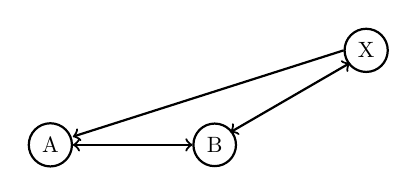
\begin{tikzpicture}[thick,scale=0.8, every node/.style={scale=0.8}]
		\draw [<->](1,1) node[anchor=east,circle,draw]{A} to (2.9,1) node[anchor=west,circle,draw]{B};
		\draw [<-](1,1.13) to (5.3,2.5) node[anchor=west,circle,draw]{X};
		\draw [<->](3.5,1.2) to (5.4,2.3);
	    \end{tikzpicture}
		
		\begin{tikzpicture}[implies/.style={double,double equal sign distance,-implies},
  			 dot/.style={shape=circle,fill=black,minimum size=2pt,
             inner sep=0pt,outer sep=2pt},thick,scale=0.8, every node/.style={scale=0.8}]
		\matrix[matrix of nodes] {
  		|[dot,label=above:$A$] (A1)| {} & [2cm] |[dot,label=above:$B$] (B1)| {} & [2cm]|[label=above:$X$] (X1)| {}\\[1cm]
  		 |[dot] (A2)| {} & [2cm] |[dot] (B2)| {} & [2cm]|[] (X2)| {}\\[1cm]
	     |[dot] (A3)| {} & [2cm] |[dot] (B3)| {} & [2cm]|[] (X3)| {}\\[1cm]
		|[dot] (A4)| {} & [2cm] |[dot] (B4)| {} & [2cm]|[] (X4)| {}\\[1cm]
  		 |[dot] (A5)| {} & [2cm] |[] (B5)| {} & [2cm]|[dot] (X5)| {}\\[1cm]
 		 |[] (A6)| {} & [2cm] |[dot] (B6)| {} & [2cm]|[dot] (X6)| {}\\[1cm]
 		 |[dot] (A7)| {} & [2cm] |[] (B7)| {} & [2cm]|[dot] (X7)| {}\\[1cm] };
	
		\draw (A1) edge[->] node[above] {M1} (B1)
	      edge[implies] (A2); 
		\draw [-latex,densely dotted](B2) edge[->] node[above] {M2} (A2);
	     \draw (A2) edge[implies] (A3);
		\draw [-latex,densely dotted](A3) edge[->] node[above] {M3} (B3);
    	  \draw (B1) edge[implies] (B2);
		\draw (B4) edge[->] node[above] {M4} (A4)
    	  edge[implies,implies-] (B3);
		\draw (B2) edge[implies] (B3);
		\draw (A3) edge[implies] (A4);
		\draw (A4) edge[implies] (A7);
		\draw (B4) edge[implies] (B6);
		%\draw [-latex,densely dashed](X5) edge[->] node[above] {DR} (A5);
		\draw (B6) edge[->] node[above] {M5} (X6);
		%\draw (X5) edge[implies] (X6);
		\draw (X7) edge[->] node[above] {M5'} (A7);
		\draw (B5) edge[implies] (B6);
		\draw (X6) edge[implies] (X7);
		\draw (A5) edge[implies] (A7);
		\end{tikzpicture} 

\end{figure}

In this scenario, the attack cooperating with a close party to complete a protocol run. Attacker $X$ overhears all messages exchanged between $A$ and $B$ during distance validation process (rapid bit-exchange), it drops message $M5$ from $B$ to $A$, then it conducts and delivers $\{r_a,r_b\}_{PK_X}$ to $A$ to complete the protocol run. As a result of that, $A$ verifies values $r_a$ and $r_b$ and accepts $X$ as a regular prover. 

\subsection{ADVSIG Vulnerability}

ADVSIG proposed by INRIA group~\cite{Raffo:2004:ASS:1029102.1029106} is a kind of secure routing protocol fortifying for OLSR~\cite{Clausen:2003:OLS:RFC3626}. In this protocol, both devices wish to declare that they have a bidirectional physical link between them. Each message in the protocol consists of three parts: a link state declared by senders, a link proof( the link state of the previous message), and a timestamp. All information is signed by sender's private key $PR$. In this protocol, $\tau_0, \tau_1,\tau_2,\tau_3$ are timestamps at each sending event; and $ASYM\_LINK$ and $SYM\_LINK$ are link states. $"A:ASYM\_LINK"$ states that $B$ is obtaining a unidirectional link to $A$ while $"A:SYM\_LINK"$ states $B$ is obtaining a bidirectional link to $A$. The protocol is presented as below.

\begin{flushleft}
 \emph{M1:} $A \to [B]: \{\O, \O, \tau_0\}_{PR_A}$\\
 \emph{M2:} $B \to [A]: \{\{"A:ASYM\_LINK", \tau_1\}_{PR_B}, \O,\tau_1\}_{PR_B}$\\
\emph{M3:} $A \to [B]: \{\{"B:ASYM\_LINK",\tau_2\}_{PR_A},\O ,\tau_2 \}_{PR_A}$\\
 \emph{M4:} $B \to [A] : \{\{"A:SYM\_LINK", \tau_3\}_{PR_B} ,\{"B:ASYM\_LINK",\tau_2\}_{PR_A} ,\tau_3\}_{PR_B}$
\end{flushleft}

Moreover, every valid link state must satisfy a maximum interval $\delta_{max}$ so that $|\tau_{s} - \tau_r | < \delta_{max}$ where $\tau_{s}$ is the value clock of the sender, and $\tau_r$ is the value clock of receiver. 

We realise that compared to OLSR specification, third message of ADVSIG changed $SYM\_LINK$ status into $ASYM\_LINK$ status. This change may affect to neighbours of $A$ if no new message from $A$ informs that $A$ owns a bidirectional link $A$ to $B$. 

Provided that the third message does not include the proof from the second one, Responder cannot ensure if Initiator has received the second message or not. As the result, internal attackers can produce the first and third messages to valid a protocol run with Responder without receiving any message from Responder. Additionally,  neighbours of Responder could be impacted by this attack due to two-hop sensing mechanism in the OLSR protocol.  Figure~\ref{advsigattack3} outlines an attacking scenario to ADVSIG where there only appears an unidirectional link X $\rightarrow$ B. Notation $->*$ describes that the messages cannot be received by $X$. 

In the attack scenario, we assume that $X$ accidentally knows the existence of $B$ out of $X$'s physical signal coverage. By using a high power antenna, $X$ can enlarge its signal range. Then $X$ emits valid messages $M1$ and $M3$ to $B$, this makes $B$ believe an existence of bidirectional physical link between $B$ and $X$.  

\begin{figure}
		\caption{ADVSIG Attack }\label{advsigattack3}
        \centering
        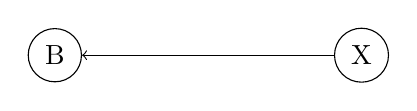
\begin{tikzpicture}
		\draw [<-](1,1) node[anchor=east,circle,draw]{B} to (4.2,1) node[anchor=west,circle,draw]{X};
		\end{tikzpicture}

	    \centering
        \begin{tikzpicture}[implies/.style={double,double equal sign distance,-implies},
  			dot/.style={shape=circle,fill=black,minimum size=2pt,
  		      inner sep=0pt,outer sep=2pt},thick,scale=0.8, every node/.style={scale=0.8}]
		\matrix[matrix of nodes] {
		  |[dot,label=above:$B$] (B1)| {} & [2cm]|[] (C1)| {}&[1cm] |[dot,label=above:$X$] (X1)| {}\\[1cm]
  		  |[dot] (B2)| {} & [2cm]|[dot,label=above:$*$] (C2)| {}& [1cm]|[dot] (X2)| {}\\[1cm]
  	      |[dot] (B3)| {} & [2cm]|[] (C3)| {}& [2cm]|[dot] (X3)| {}\\[1cm]
 		  |[dot] (B4)| {} & [2cm]|[dot,label=above:$*$] (C4)| {}& [1cm]|[] (X4)| {}\\
		};
		\draw (X1) edge[->] node[above] {M1} (B1)
	      edge[implies] (X3); 
		\draw (B2) edge[->] node[above] {M2} (C2)
	      edge[implies,implies-] (B1);
		\draw (B3) edge[<-] node[above] {M3} (X3)
    	  edge[implies,implies-] (B2);
		\draw (B4) edge[->] node[above] {M4} (C4)
    	  edge[implies,implies-] (B3);
		\end{tikzpicture}

\end{figure}

We found the same problem in the work~\cite{Adnane20131159}. Authors proposed a trusted-based security for OLSR protocols where all participants must trust together. However, internal attackers can successfully create a fake bidirectional physical link to a target as they do in ADVSIG. 

\section{Correctness of ADVSIG}
In this part, we would like to propose a simple correctness of ADVSIG scheme. We attach link proofs for the second and the third message. Thus, the first link proof in the second message is a hash of the first message encrypted by B's public key, while the second link proof in the third message is the link state of the previous one. 

$A$'s signature wrapped by hash function is impossible to be reproduced by any attacker. As the result of that, even the attacker incidentally receives the message of $B$, he cannot create a correct reply. The scheme is presented as follows. 

\begin{flushleft}
 \emph{M1:} $A \to [B]: \{\O, \O, \tau_0\}_{PR_A}$\\
 \emph{M2:} $B \to [A]: \{\{"A:ASYM\_LINK", \tau_1\}_{PR_B},$ $h(\{\{\O, \O, \tau_0\}_{PR_A}\}_{PR_B}),\tau_1\}_{PR_B}$\\
\emph{M3:} $A \to [B]: \{\{ "B:SYM\_LINK",\tau_2\}_{PR_A},$ $\{"A:ASYM\_LINK", \tau_1\}_{PR_B},\tau_2\}_{PR_A}$\\
 \emph{M4:} $B \to [A] : \{\{ "A:SYM\_LINK", \tau_3\}_{PR_B},$ $\{"B:SYM\_LINK",\tau_2\}_{PR_A} ,\tau_3\}_{PR_B}$
\end{flushleft}

\section{Formal Analysis of Neighbour Discovery Protocol}

As mentioned in the previous chapter, the problem existing in current secure neighbour discovery protocols associates to the incorrect ranging and validating processes which usually lies on some physical characteristics such as location, timestamp, and physical signal range. Meanwhile, existing formal models are partly facilitated with these characteristics to cope with the discussing problems. Therefore, in this section, we are going to produce a formalism to cover limitations of current formal model. To begin with, we will present related work and point out their limitations. 

\subsection{Related Work on Physical Characteristic Modelling}

Most current approaches formalised time as timestamps to determine key-expiration~\cite{Li:2007:ESS:1338438.1338469} , and integrity of messages via round trip time-of-flight~\cite{Poturalski:2008:TPS:1456396.1456400, RaphaelJamet}. Meanwhile, location information was considered in problems of correctness of routing protocols~\cite{5230621,Basin:2009:LGP:1616077.1616079}, or evaluating distance between two neighbours in~\cite{Poturalski:2008:TPS:1456396.1456400}. Barely found in literature, signal characteristic is an interesting feature mentioned in~\cite{Poturalski:2008:TPS:1456396.1456400}. However, this feature is not truly helpful to reveal attacking location and direction. 

Close to our approach, the models~\cite{Yang03modelingvulnerabilities, 4481351} extended Strand Spaces to pick up vulnerabilities in ad-hoc routing protocols while other approaches~\cite{Li:2007:ESS:1338438.1338469, Sharp:2007:TTS:2391910.2391948} expressed temporal phenomena, and notably key-expiration. In addition to, metric strand proposed in~\cite{Thayer:2010aa} was presented to deal with locale authentication. Nevertheless, no specified attack and proof was provided in this work. 

\subsection{Assumptions}\label{assumptions}

Before presenting our model extensions of Strand Spaces, we formulate some supplementary assumptions concerning physical characteristics of wireless interfaces and environment, that we will have to take into account. We explicitly declare some reasonable assumptions as follows:

\begin{itemize}
\item Every participant is equipped with: (I) \textit{various types of wireless devices with different signal powers}, (ii) \textit{precise clock devices}. To make simplicity, radiation power is assumed to stay constantly during protocol execution.
\item An \textit{idealized communication environment} is regarded where wireless signal travels on non-obstacle path with speed of light $v_c$. Following this assumption, when a participant stands on signal propagation region of others, he can listen to their exchanged messages. 
\item A \textit{secure key distribution function} is enabled on all participants. 
\end{itemize}

Furthermore, our current work only focuses on \textit{a static wireless network model} where devices do not change their position due to complexity of modelling dynamic networks. Dynamic network, hence, could be extended and considered in our future work. 

\subsection{Wireless Strand Spaces}

Obviously, original Strand Spaces was designed for cryptographic protocols, so it apparently cannot analyse neighbour discovery protocols. To tackle this limitation, we facilitate Strand Spaces model with our extensions to account for wireless context, then we call the \textit{wireless Strand Spaces}. In particular, a node in our model is equipped with \textit{location, timestamp, signal range} information. Location shows where the node is standing, timestamp indicates when a node happens, and signal range refers to how far the wireless signal of the node can reach. As consequence, the definition of a wireless node is presented as below.

\begin{Definition}[Wireless Node] A \emph{wireless node} $n$ is a tuple of $(t, l_n, \tau_{n}, R_n)$ where $t$ is a signed term, $l_n$ is location, $\tau_{n}$ is a timestamp, and $R_n$ is signal range.\end{Definition}

Note that, $l_n$, \textit{location of a node n}, is extensible to any Euclidean space. \textit{Distance between nodes} $n$ and $n'$ is noted as $dist(n,n')$. \textit{Timestamp}, $\tau_{n}$, appears in a node to check freshness property, and it is a value of local clock when an event begins. \textit{Signal range of a node n}, $R_n$, is a positive real number. According to assumption~\ref{assumptions}, signal power does not change during a protocol execution; hence, we denote $R_{st}$ is physical signal  propagation of strand $st$. 

In realistic scenarios, there always exists a gap between two events, so a fixed value $\delta_{tp}$ is noted as a \textit{processing delay} of edge $ (+n) \Rightarrow (-n')$. We continue describing definitions of wireless strand, and wireless bundle. 

\begin{Definition}[Wireless Strand] A \emph{wireless strand} is a strand with wireless nodes.
\end{Definition}

Recall that static network is being discussed in this thesis; hence, a strand with fixed location is so-called \textit{a fixed wireless strand}. Thus, all nodes in a fixed strand share the same location. We denote $loc(st)$ be the location of strand $st$, and $dist(st,st')$ be the distance between two strands $st$ and $st'$. To avoid ambitious notions, notion of strand in this section is now refer to a wireless strand. 

Existence of a physical link is usually hard to be precisely criticised due to environment complexity. Hence, in this work, a physical link is simply determined by a distance value among participants. Another speaking, by any mean, a bidirectional physical link exists between two participants if and only if the distance between them is lower than their own signal coverage. We formally define notations of links as follows. Noted that, the notation $ \rightarrow^* n'$, referred from the original Strand Spaces, means that there is a path of a term from node $n$ to node $n'$.  

\begin{Definition}[Definition of Links]
\begin{itemize}
\item \emph{Unidirectional physical link}:  \\ $\forall st,st' \in \mathcal{B}$, $plink(st,st', \rightharpoonup) \Leftrightarrow$ $dist(st,st') \le R_{st}$.
\item \emph{Bidirectional physical link}: \\ $\forall st,st' \in \mathcal{B}$, $plink(st,st', \rightleftharpoons) \Leftrightarrow$ $(dist(st,st') \le R_{st}) \wedge (dist(st',st) \le R_{st'})$.
\item \emph{Unidirectional logical link}: \\ $\forall st, st' \in \mathcal{B}, n \in st, n' \in st', \exists (n_1 \rightarrow^* n_2) \Leftrightarrow \exists link(st, st',\rightharpoonup)$.
\item \emph{Bidirectional logical link}: \\ $\forall st, st' \in \mathcal{B},$ $ \exists link(st, st',\rightharpoonup) \wedge \exists link(st', st,\rightharpoonup) \Leftrightarrow \exists link(st, st',\rightleftharpoons)$.
\end{itemize}	
\end{Definition}

\subsection{Extended Penetrator Model}\label{penndp2}

Along with Dolev-Yao penetrator model~\cite{dolev-yao}, this thesis considers two physical attacks: relaying attack and link spoofing attack. These attacks are apparently conducted from a sequence of atomic events such as sending events with high a power antenna  and single relaying events respectively. Hence, we encode the atomic malicious actions into two new penetrator strands. Precisely, given penetrator strand $st_p$, and $n, n' \in st_p$. 
\begin{itemize}
\item [SRL.] \emph{Single relay:} \\ $\langle -(t, l_n, \tau_{n}, R_n), +(t, l_n', \tau_{n'}, R_{n'}) \rangle >$ where $\tau_{n'} - \tau_{n} = 0$.
\item [BS.] \emph{Boosting signal:} $\langle +(t, l_n, \tau_{n}, R_M) \rangle$ where $R_M$ could be an unlimited value. 
\end{itemize}

At present, single relaying attack is possibly detected by advanced protection mechanisms presented in the previous section. Therefore, we consider the \emph{weak penetrator model} which does not deal with relaying attack. In contrast, \emph{strong penetrator model} has full attacker's capabilities. 

\subsection{Secure Neighbour Discovery Goal}

We express formally secure neighbour discovery goals in Strand Spaces model as an authentication goals:

\emph{Secure Neighbour Discovery Goal:} \textit{For all bundles $\mathcal{B}$, two roles $R, R' \in \mathcal{B}$, and strand $st$, there exists a strand $st$' such that if $st \in R$ has $ \mathcal{B}_{height}$ i, and some protocol assumptions hold then $st' \in R'$ has $\mathcal{B}_{height}$. Moreover, there exists a physical link $plink(st,st',\rightleftharpoons)$.}

Guttman stated that analysing authentication properties of a protocol means finding right choices for $R$ and $R'$ for $i$, and $j$, and necessary origination assumptions. However, this proving way could extremely cost time and effort when solving a complicated protocol. So, to ease this job, Guttman introduced authentication tests~\cite{authenticationtests} as supporting tools. In this test, there indeed exists a bidirectional logical link between two regular strands so that they can communicate to each other.

Following to this idea, we construct our authentication link tests to guarantee whether a protocol satisfies the goal or not.  At first, we introduce a link test edge, and an authentication logical link test. Then, we conduct authentication physical link tests based on time and location estimation. 

\subsection{Logical Link Tests}

To get rid of link spoofing attack, a protocol should support a mechanism enabling a participant to verify whether his protocol-mate has already seen its messages or not. As a solution, challenge-respond mechanisms, described formally as authentication tests, could be used in which a participant delivers a random as a challenge and receives an answer only produced by an intended sender. The answer usually contains a cryptographic part as a proof that allows the participant verifies origin, integrity, or confidentiality of this message. 

One possible particular proof, called \textit{hidden proof}, is a nonce encrypted by pre-shared key or by public key of Initiator, or a hash of nonce and name of Responder. Another one, called \textit{clear proof}, is a part of previous Initiator's message that contains Responder's ID and a timestamp, and is signed by private key of the Initiator. We define notations of \emph{identification factor}, and a \emph{provable component} to express these such proofs. 

\begin{Definition} \emph{An identification factor} in a component $\{c\}_k$ is:
\begin{itemize}
	\item(clear-form) \emph{Responder's $ID_{Res}$ and a timestamp t} such that $(ID_{Res} \sqsubseteq \{c\}_k ) \wedge (t \sqsubseteq \{c\}_k)$ in which $k$ is a private key of Initiator. Or, 
	\item(hidden-form) \emph{a nonce N} such that N $\sqsubseteq \{c\}_k$ in which $k$ is a pre-shared secret key or public key of Responder.\end{itemize}
\end{Definition}

\begin{Definition}\emph{A provable component} is a component which has one of forms:
\begin{itemize}
	\item (clear-form):$\{m\}_{PR_{Res}}$ in which $idf \sqsubseteq \{c\}_{PK_{Init}} \sqsubseteq m$ where $PR_{Res}$ is a private key of Responder, and $PK_{Init}$ is the public key of Initiator;  
	\item (hidden-from):$\{m\}_k$ or $\{h(m)\}_{PK_{Res}}$ in which $idf \sqsubseteq m$, and $k$ is a pre-shared key, and $PK_{Res}$ is a public key of Responder;
\end{itemize}
\end{Definition}

We conduct \emph{a logical link test}, and \emph{an authentication logical link test} which allows a participant to ensure that none of it's partners completes a protocol run without receiving its messages. We would like to revise the definition of \emph{a test} defined in~\cite{authenticationtests}. 

\begin{Definition}[A test] 
$t = \{m\}_k$ is \emph{a test} for $a$ in $n$ if:
\begin{enumerate}
\item $a\sqsubseteq t$ and $t$ is a component of $n$;
\item The term $t$ is not a proper subterm of a component of any regular node $n' \in \Sigma$. 
\end{enumerate}
The edge $n \Rightarrow^+ n'$ is \emph{a test} for $a$ if $a$ uniquely originates at $n$ and $n \Rightarrow^+ n'$ is a transformed edge for $a$. 
\end{Definition}

\begin{Definition}[Logical Link Test] The edge $n \Rightarrow^+ n'$ is a \emph{logical link test} for an identification factor $idf$ in $t = \{m\}_k \sqsubseteq term(n')$ if it is a test for $idf$ in which $k \not\in P$ and $t$ is a provable component for $idf$ in $n'$
\end{Definition}

The authentication logical link test below results a bidirectional logical link between two strands $st$ and $st'$ in a bundle. 
\begin{Proposition}[Authentication Logical Link Test]\label{logicaltest}Let $n \Rightarrow^+ n' \in st$ be a logical link test for an identification factor $idf \sqsubseteq t' \sqsubseteq term(n')$. There exist regular nodes $m, m' \in st'$ such that $t'$ is a provable component of $m'$, and $m \Rightarrow^+ m'$ is a transforming edge for $idf$. 
\end{Proposition}

\begin{proof}
Reusing the proof of proposition 20 in~\cite{Guttman:2002:ATS:568264.568267}, we obtain regular edge $m \Rightarrow m'$ in a regular $st'$. On one hand, identification factor $idf$ allows $st'$ to ensure the existence of $st$ in the protocol. On the other hand, a new provable component as well helps $st$ ensure $st'$ has already received $idf$. As a result, Initiator can ensure existence of a bidirectional logical link $link(st,st',\rightleftharpoons)$ with Responder. 
\end{proof}

\subsection{Authentication Physical Link Tests}

In this sub-section, distance between two neighbours can be estimated through message time-of-flight in, or location between two nodes in a direct logical link test edge $n \Rightarrow n'$ ($\Rightarrow$ instead of $\Rightarrow^+$), or DE edge, for an identification factor $idf$. So, we introduce two authentication physical link tests: time-based and location-based authentication tests. 

\subsubsection*{Time-based authentication test}

Basically, distance between two participants can be determined by message travelling time. Formally speaking, the proposition below describes this idea.

\begin{Proposition}\label{difrange}
Consider a weak penetrator model, regular strands $st, st' \in \mathcal{B}$, nodes $n,n' \in st$, and $(+n) \Rightarrow (-n')$ is a DE edge for an identification factor $idf$. If $(\tau_{n'} - \tau_{n})\div 2 \le R_{st} \div v_c + \delta_{tp} \div 2$, then $\exists plink(st,st',\rightleftharpoons)$. 
\end{Proposition}

\begin{proof}

According to the proposition~\ref{logicaltest}, there is a bidirectional logical link between $st$ and $st'$. Furthermore, in absence of relaying attack, to receive message from $st'$, $st$ must stand within physical signal region of $st'$. As a result, we have $R_{st'} \wedge R_{st}$ (1). We then calculate the travelling time of $idf$ between node $n$ and $n'$. 
\begin{equation*}
\begin{split}
  	 \tau_{n'} - \tau_{n} \ge \frac 1 {v_c}(dist(n,m) + dist(m', n')) + (\tau_{m'} - \tau_{m}) \\ \Leftrightarrow 
	 \tau_{n'} - \tau_{n} \ge 2 \times \frac 1 {v_c}(dist(n,m)) + \delta_{tp} \\ \Leftrightarrow 
	 \frac 1 {2} (\tau_{n'} - \tau_{n}) \ge \frac 1 {v_c} dist(st,st') + \frac 1 {2} \delta_{tp} 
\end{split}
\end{equation*}

Additionally, according to proposition assumption, we have $ \frac 1 {2} (\tau_{n'} - \tau_{n}) \le \frac 1 {v_c} R_{st} + \frac 1 {2} \delta_{tp} $ (2). From (1) and (2), we conclude $dist(st,st') \le R_{st} \le R_{st'} $. Eventually, there exists a physical link between $st$ and st'.
\end{proof}

In case of strong penetrator model, we need a strong assumption on similarity of signal ranges of all principals. The physical link, hence, could be obtained as below proposition. 

\begin{Proposition}\label{samerange}
Given regular strands $st, st' \in \mathcal{B}$, assume that $R_{st} = R_{st'}$, $\exists link(st,st', \rightleftharpoons)$, nodes $n,n' \in st$, and $(+n) \Rightarrow (-n')$ is a DE edge for an identification factor $idf$. If $(\tau_{n'} - \tau_{n})\div 2 \le R_{st} \div v_c + \delta_{tp} \div 2$, then $\exists plink(st,st',\rightleftharpoons)$. 
\end{Proposition}
\begin{proof}

Using the proof of proposition~\ref{difrange}, we have $(\tau_{n'} - \tau_{n}) \ge \frac 1 {v_c} dist(st,st') + \frac 1 {2} \delta_{tp}$. Additionally, since $R_{st} = R_{st'}$, we can conclude $dist(st,st') \le R_{st}$ $\cup$ $dist(st,st') \le R_{st'}$. Eventually, there exists a physical link between $st$ and st'. 

\end{proof}

However, when removing the assumption $R_{st} = R_{st'}$ in proposition~\ref{samerange}, we discover a flaw in the time-based authentication test. Let's analyse the problem into sub-cases:

\emph{Case 1}: $R_{st} \ge dist(st,st')$ and $R_{st'} \ge dist(st,st')$. Obviously, both $st$ and $st'$ can receive messages of each other. 

\emph{Case 2}: $R_{st} \le dist(st,st')$ and $R_{st'} \le dist(st,st')$. Let's call $\Delta_d = dist(st,st') - R_{st}$, we calculate the message travelling time between $n$ and $n'$ as follows: 
\begin{equation*}
\begin{split}
	 \tau_{n'} - \tau_{n} \ge \frac 1 {v_c}(dist(n,m) + dist(m', n')) + (\tau_{m'} - \tau_{m}) \\ \Leftrightarrow
	\tau_{n'} - \tau_{n} \ge 2 \times \frac 1 {v_c} dist(n,m) + \delta_{tp}  \\
\Leftrightarrow	\tau_{n'} - \tau_{n} \ge 2 \times \frac 1 {v_c}(R_{st} + \Delta_d) + \delta_{tp} \\
\Leftrightarrow	2 \times \frac 1 {v_c} R_{st} + \delta_{tp} \ge 2 \times \frac 1 {v_c} (R_{st} + \Delta_d) + \delta_{tp} \\
\Leftrightarrow	0 \ge 2 \times \frac 1 {v_c} \Delta_d 
\end{split}
\end{equation*}
The last equation is a contradiction when $\Delta_d$ is larger than zero, so this case will not happen. 

\begin{figure}
	\caption{Link spoofing: Case 3} \label{chap3case3}
	\centering
	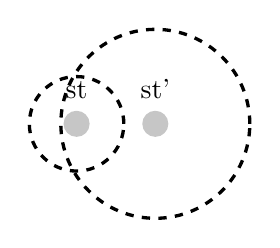
\begin{tikzpicture}
		\begin{scope}[very thick,dashed]
		\draw (0,1) circle (.6cm);
		\draw (0,1) node[circle,fill=gray!45,label=above:st]{};
		\draw (1,1) circle (1.2cm);t
		\draw (1,1) node[circle,fill=gray!45,label=above:st']{};
		\end{scope}
	\end{tikzpicture}
\end{figure}
		
\begin{figure}
    \caption{Link spoofing: Case 4} \label{chap3case4} 
    \centering
	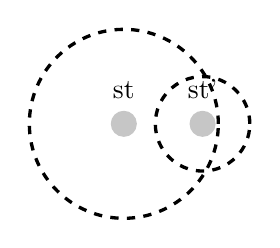
\begin{tikzpicture}
		\begin{scope}[very thick,dashed]
		\draw (0,1) circle (1.2cm);
		\draw (0,1) node[circle,fill=gray!45,label=above:st]{};
		\draw (1,1) circle (0.6cm);
		\draw (1,1) node[circle,fill=gray!45,label=above:st']{};
		\end{scope}
	\end{tikzpicture}

\end{figure}

\emph{Case 3}: $R_{st} \le dist(st,st')$ and $R_{st'} \ge dist(st,st')$. Let's call $\Delta_d = dist(st,st') - R_{st}$, we calculate the message travelling time between $n$ and $n'$ as follows: 
\begin{equation*}
\begin{split}
		\tau_{n'} - \tau_{n} \ge \frac 1 {v_c}(dist(n,m) + dist(m', n')) + (\tau_{m'} - \tau_{m}) \\ \Leftrightarrow
		\tau_{n'} - \tau_{n} \ge 2 \times \frac 1 {v_c}(dist(n,m)) + \delta_{tp}\\ \Leftrightarrow
		\tau_{n'} - \tau_{n'} \ge 2 \times \frac 1 {v_c} (R_{st} + \Delta_d) + \delta_{tp} \\ \Leftrightarrow
		2 \times \frac 1 {v_c} R_{st} + \delta_{tp} \ge 2 \times \frac 1 {v_c} (R_{st} + \Delta_d ) + \delta_{tp} \\ \Leftrightarrow
		0 \ge \delta_{d} 
\end{split}
\end{equation*}
The only possible case is $\Delta_{d}$ equals zero, but it is too trivial. Otherwise, a fast relaying attack occurs at the side from $st$ to $st'$. Case 3 is presented at figure~\ref{chap3case3}.

\emph{Case 4}: $R_{st} \ge dist(st,st')$ and $R_{st'} \le dist(st,st')$. Presented at the figure~\ref{chap3case4}, it similarly happens as case 3. If $R_{st}$ is much larger than $dist(st,st')$, then a fast relaying attack occurs at the side from $st'$ to $st$. 
%---------------------------Location-based-----------------------%
\subsubsection*{Location-based authentication test}

Location information can help to determine the distance between two strands. Hence, we formally describe location-based authentication test using knowledge of participant locations. 

\begin{Proposition}
Consider a weak penetrator model, and location information is confidentially exchanged and stored. Given strands regular $st, st' \in \mathcal{B}$, and $\exists link(st,st', \rightleftharpoons)$, and let $d = |loc(st),loc(st')|$ be a distance between two location of $st$ and $st'$, if $d \le R_{st}$ and $d\le R_{st'}$ , then $\exists plink(st, st',\rightleftharpoons)$. 
\end{Proposition}

\begin{proof}
  
Obviously, we have $|loc(st),loc(st')| = dist(st,st')$, then $dist(st,st') \le R_{st}$ and $dist(st,st') \le R_{st'}$. As a result, there exists a physical link between $st$ and st'. 

\end{proof}

Note that, without assumption on trusted location information, the location-based protocols may contain flaws in some cases. For instance, $st$ could not address correctly the physical location of $st'$ , then an attacker uses his knowledge about location of $st$ to make a fake link between them. Furthermore, location-based protocols share the same trouble with time-based protocols when analysed in our strong penetrator model. 

%-----------------------------------------------------------------------------------------------------------------------------------------------------------------------------%

\section{Analysis of ADVSIG}

In ADVSIG protocol, a node wishes to detect neighbours with bi-directional physical links. The protocol is presented as below. 
\begin{flushleft}
 \emph{M1:} $A \to [B]: \{\O, \O, \tau_0\}_{PK_A}$\\
 \emph{M2:} $B \to [A]: \{\{"A:ASYM\_LINK", \tau_1\}_{PK_B}, \O,\tau_1\}_{PK_B}$\\
\emph{M3:} $A \to [B]: \{\{"B:ASYM\_LINK",\tau_2\}_{PK_A},\O ,\tau_2 \}_{PK_A})$\\
 \emph{M4:} $B \to [A] : \{\{"A:SYM\_LINK", \tau_3\}_{PK_B} ,\{"B:ASYM\_LINK",\tau_2\}_{PK_A} ,\tau_3\}_{PK_B})$
\end{flushleft}

We analyse ADVSIG protocol to show usefulness of our model. There are three kinds of strands in ADVSIG protocol:

\begin{Definition}
An infiltrated Strand Spaces $(\Sigma,\mathcal{B})$ is a model of ADVSIG protocol if $\Sigma$ is the union of three following kind of strands:
\begin{itemize}
\item \emph{Penetrator strands} $st_p \in \mathcal{B}$,
\item \emph{Initiator strand} with strand: {\footnotesize $st =  \{\langle st, 1 \rangle,\langle st, 2 \rangle,\langle st, 3 \rangle,\langle st, 4 \rangle\} \in Init[A,\tau_0,\tau_2]$}, with trace $<+M_1, -M_2 , +M_3,-M_4>$.
\item \emph{Responder strand} with strand: {\footnotesize $st' = \{\langle st', 1 \rangle,\langle st', 2 \rangle,\langle st', 3 \rangle,\langle st', 4 \rangle\} \in Resp[B,\tau_1,\tau_3]$}, with trace $<-M_1, +M_2 , -M_3,+M_4>$.
\end{itemize}
\end{Definition}

Protocol assumption: 
\begin{itemize}
\item ps1: $|\tau_{s} - \tau_r| \le \delta_{max}$
\item ps2: Time synchronisation mechanism is set on participants.
\end{itemize}

\subsubsection*{Initiator's Guarantee} 

Initiator states the guarantee as follows.

\emph{
Suppose $\mathcal{B}$ is a wireless bundle. Under the conditions $ps1$ and $ps2$, if $\mathcal{B}$ contains a strand $st \in Init[A,B,\tau_0,\tau_1,\tau_2,\tau_3]$ with $\mathcal{B} -height$ 4, then $\mathcal{B}$ contains a strand $st' \in Resp[A,B,\tau_0,\tau_1,\tau_2,\tau_3]$ with $\mathcal{B} -height$ 4. Moreover, there exists a $plink(st,st',\rightleftharpoons)$. 
}

Mechanically, to find out if the statement is correct or not, we start asserting the logical link guarantee between two participants. Let's call node $n_1$,  $n_2$, $n_3$ and $n_4$ be $\langle st,1\rangle$, $\langle st,2\rangle$, $\langle st,3\rangle$, and $\langle st,4\rangle$ respectively. 
 
\emph{Logical link guarantee}: At first, we search for a DE edge with an identification factor:
\begin{itemize}
\item The edge $n_1 \Rightarrow n_2$ does not contain any identification factor in the challenge message. 
\item The edge $n_3 \Rightarrow n_4$ : $term(n_3)$ contains a clear-form identification factor which is response's name $B$ and a timestamp $\tau_2$, all signed by A's private key, and $term(n_4)$ embodies the a clear-form provable component $\{\{ "A:SYM\_LINK", \tau_3\}_{PK_B} ,\{ "B:ASYM\_LINK",\tau_2\}_{PK_A} ,\tau_3\}_{PK_B}$.
\end{itemize}

The edge $n_3 \Rightarrow n_4$ satisfies the authentication logical link test. Therefore, $A$ can verify a logical link between $A$ and $B$, and $B$ is a regular party. To find out if there exists $plink(st,st,\rightleftharpoons)$, we apply the time-based authentication test.  

\emph{Physical link guarantee}: To verify the distance between $st$ and $st'$, we apply the time-based authentication test for the edge $n_3 \Rightarrow n_4$. Let call $\tau_{n_4}$ be the timestamp of node $n_4$. 


The test concludes that if $(\tau_{n_4} - \tau_2) \div 2 \le R_{st} \div c$ + $\delta_{tp} \div 2$ (1) then $\exists plink(st,st', \rightleftharpoons)$. Let's call node $n'_3$ and $n'_4$ be $\langle st',3\rangle$, and $\langle st',4\rangle$ respectively. And let $\tau_{n'_3}$ be the timestamp of node $n'_3$. 

Basing on assumption ps1 and ps2, we calculate the message travelling time from node $n_3$ to $n_4$:
\begin{equation*}
\label{equation1}
\begin{split}
\tau_{n_4} - \tau_2 = \\
(\tau_{n'_3} - \tau_2) + (\tau_3 - \tau_{n'_3}) + (\tau_{n_4} - \tau_3) \\
\Rightarrow \tau_{n_4} - \tau_2 \le 2 \times \delta_{max} + \delta_{tp} (2)
\end{split}
\end{equation*}

 Let $2\times(1) - (2)$, we have
\begin{equation*}
\label{equation2}
\begin{split}
	R_{st} \div v_c - \delta_{max} \ge 0 (3)
\end{split}
\end{equation*}

If inequality (3) holds, then $\exists plink(st,st', \rightleftharpoons)$. $\qed$
  
\subsubsection*{Responders Guarantee}

Initiator states the guarantee as follows.
\emph{
Suppose $\mathcal{B}$ is a wireless bundle. Under the conditions $ps1, ps2$, if $\mathcal{B}$ contains a strand $st' \in Resp[A,B,\tau_0,\tau_1,\tau_2,\tau_3]$ with $\mathcal{B} -height$ 4, then $\mathcal{B}$ contains a strand $st \in Init[A,B,\tau_0,\tau_1,\tau_2,\tau_3]$ with $\mathcal{B} -height$ 4. Moreover, there exists a $plink(st,st',\rightleftharpoons)$. 
}

The proof of this statement is quite identical to Initiator's guarantee. However, when looking for a bidirectional logical link, regrettably, we cannot find any logical link test edge in Responder strand. As a result, $B$ can be a victim of spoofing attack. $\qed$ 
 
\subsubsection*{Link spoofing attack on ADVSIG} 

Formally speaking, since $n_1$ and $n_3$ do not contain any proof of reception, they possibly lie on $X$ strand. Actually, when $X$ accidentally knows the existence of $B$ but it cannot listen to $B$, $X$ persuades $B$ that $B$ will own a bidirectional physical link with $X$ by following strand.  
\begin{flushleft}
$st_x = \{(M_1,loc(st_X),\tau_{x1}, R_M) ,(M_3,loc(st_X)$ $,\tau_{x3}, R_M)\}$ $\in$ $Init[X,\tau_{x1},\tau_{x3}]$ with trace $<+M_1,+M_3>$.
\end{flushleft}

\section{Conclusion}

This chapter has addressed a serious problem of current neighbour discovery protocols that have not introduced before. The problem comes when participants use wireless interfaces with different signal power, that leads the secure neighbour discovery protocols cannot correctly verify the distance between participants. Moreover, some of them were vulnerable to internal attackers due to incorrectly validating physical links.     

We extended the original Strand Spaces model to be able to analyse secure neighbour protocols. To achieve this, we modified the model so that it becomes possible to take into account some physical properties including timestamp, location, and signal range. The penetrator model has been adapted in consequence. Thank our model, time-based, even location-based neighbour discovery techniques were formally proved that they would not guarantee the existence of physical bidirectional links. 

Concerning future work, we will first try to extend the model in order to capture mobility and network topology. In a second step, we plan to study how we could automate the analysis procedure.
